%%%%%%%%%%%%%%%%%%%%%%%%%%%%%%%%%%%%%%%%%%%%%%%%%%%%%%%%%%%%%%%%%%%%%%
% Problem statement
\begin{statement}[
  problempoints=110,
  timelimit=5 sekundi,
  memorylimit=512 MiB,
]{Klasika}

%\setlength\intextsep{-0.1cm}
%\begin{wrapfigure}[9]{r}{0.17\textwidth}
%\centering
%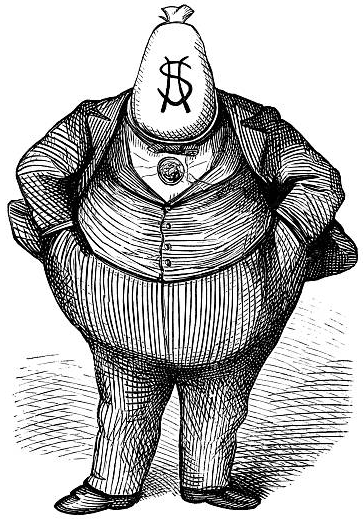
\includegraphics[width=0.17\textwidth]{img/holding.png}
%\end{wrapfigure}

,,\textit{Klasična subota amigosi, jučer jedan nemili klasikus metlikus, a danas\dots}''
-- Romano Obilinović, prvi strijelac slovenske lige 2001. i 2005.,
legenda interneta, kralj kladionica.

Klasična glazba u razgovornom je govoru pojam koji označava vrstu glazbe
sviranu klasičnim instrumentima, ali se ustvari radi o vrsti glazbe koja
potječe iz razdoblja klasicizma. Klasična gimnazija naziv je za srednju školu
u kojoj se u toku čitavog školovanja uče klasični jezici (latinski i grčki).
Razdoblje klasične književnosti\dots

Isprike, autor se malo zanio, nije lagano napisati \textit{neklasičan} tekst
za ovako klasičan zadatak. Slijedi klasičan tekst.

U početku bijaše čvor s oznakom $1$ koji je ujedno i korijen stabla. Na vama je
da podržite $Q$ upita oblika:
\begin{itemize}
  \item \texttt{Add x y} -- Dodaje u stablo novi čvor kao dijete čvora $x$. Taj
        je novi čvor sa čvorom $x$ povezan bridom težine $y$, a njegova je oznaka
        jednaka broju čvorova koji se sada nalaze u stablu.
  \item \texttt{Query a b} -- Pronalazi duljinu najduljeg puta koji započinje u
    čvoru $a$, a završava u nekom od čvorova podstabla čvora $b$ (smatramo da je i
    čvor $b$ dio svoga podstabla). Duljinu puta definiramo kao isključivo ili
    (xor) težina svih bridova koji se nalaze na putu.
\end{itemize}

%%%%%%%%%%%%%%%%%%%%%%%%%%%%%%%%%%%%%%%%%%%%%%%%%%%%%%%%%%%%%%%%%%%%%%
% Input
\subsection*{Ulazni podaci}
U prvom je retku prirodan broj $Q$ $(1 \le Q \le 200\ 000)$ iz teksta zadatka.

U $i$-tom od sljedećih $Q$ redaka nalazi se $i$-ti upit koji formatom odgovara
nekom od upita iz teksta zadatka. Vrijednosti $x$, $a$ i $b$ u svakom će
upitu odgovarati čvoru koji u tom trenutku postoji, a vrijednost $y$ bit će
manja ili jednaka $2^{30}$.

%%%%%%%%%%%%%%%%%%%%%%%%%%%%%%%%%%%%%%%%%%%%%%%%%%%%%%%%%%%%%%%%%%%%%%
% Output
\subsection*{Izlazni podaci}
Potrebno je ispisati odgovor na svaki upit tipa \texttt{Query}. Svaki je
odgovor potrebno ispisati u zasebnom retku onim redoslijedom kojim se
odgovarajući upiti pojavljuju u ulazu.

%%%%%%%%%%%%%%%%%%%%%%%%%%%%%%%%%%%%%%%%%%%%%%%%%%%%%%%%%%%%%%%%%%%%%%
% Scoring
 \subsection*{Bodovanje}
{\renewcommand{\arraystretch}{1.4}
  \setlength{\tabcolsep}{6pt}
  \begin{tabular}{ccl}
 Podzadatak & Broj bodova & Ograničenja \\ \midrule
  1 & 11 & $Q \le 200$ \\
  2 & 22 & $Q \le 2\ 000$ \\
  3 & 33 & U svim upitima tipa \texttt{Query} vrijedi $b=1$ \\
  4 & 44 & Nema dodatnih ograničenja.
\end{tabular}}

%%%%%%%%%%%%%%%%%%%%%%%%%%%%%%%%%%%%%%%%%%%%%%%%%%%%%%%%%%%%%%%%%%%%%%
% Examples
\subsection*{Probni primjeri}
\begin{tabularx}{\textwidth}{X'X'X}
\sampleinputs{test/klasika.dummy.in.1}{test/klasika.dummy.out.1} &
\sampleinputs{test/klasika.dummy.in.2}{test/klasika.dummy.out.2} &
\sampleinputs{test/klasika.dummy.in.3}{test/klasika.dummy.out.3}
\end{tabularx}

%%%%%%%%%%%%%%%%%%%%%%%%%%%%%%%%%%%%%%%%%%%%%%%%%%%%%%%%%%%%%%%%%%%%%%
% We're done
\end{statement}

%%% Local Variables:
%%% mode: latex
%%% mode: flyspell
%%% ispell-local-dictionary: "croatian"
%%% TeX-master: "../hio.tex"
%%% End:
